\documentclass[border=5mm]{standalone}
\usepackage{tikz}
\makeatletter
\tikzset{
    dot diameter/.store in=\dot@diameter,
    dot diameter=1pt,
    dot spacing/.store in=\dot@spacing,
    dot spacing=5pt,
    dots/.style={
        line width=\dot@diameter,
        line cap=round,
        dash pattern=on 0pt off \dot@spacing
    }
}
\makeatother
\begin{document}
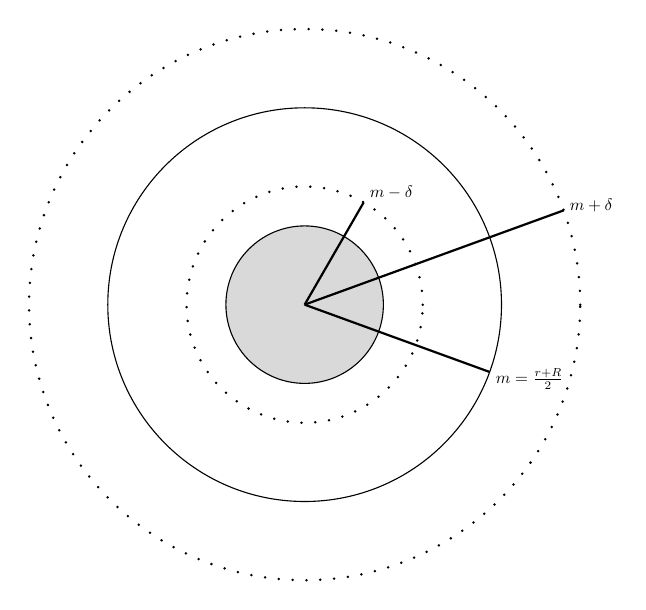
\begin{tikzpicture}[
  every node/.style={scale=0.6}
]
% inner/outer circle:
\filldraw [fill=gray!30, draw=black] (0,0) circle[radius=1];


% bug: when \k=0, dot spacing=0pt, the dots disappear!
% circle added outside the loop as a fix
\foreach \n in {1,2,3} {
  \pgfmathsetmacro{\radius}{\n+0.5}
  \pgfmathtruncatemacro{\k}{abs(\n-2)}
  \draw [black, dot diameter=1pt, dot spacing=\k*5pt, dots] (0,0) circle[radius=\radius];
}
  \draw [black] (0,0) circle[radius=2.5];
  \draw [thick] (0,0) -- (60:1.5cm) node[anchor=200] {$m-\delta$};
  \draw [thick] (0,0) -- (20:3.5cm) node[anchor=190] {$m+\delta$};
  \draw [thick] (0,0) -- (-20:2.5cm) node[anchor=170] {$m=\frac{r+R}{2}$};

\end{tikzpicture}
\end{document}